\documentclass[a4paper,11pt]{article}
\usepackage[T1]{fontenc}
\usepackage{fullpage,graphicx,psfrag,amsmath,amsfonts}
\usepackage[utf8]{inputenc}
\usepackage[english]{babel}
\usepackage{lipsum}
\usepackage{url}
\usepackage{amsmath}
\usepackage{bm}
\usepackage{listings}
\usepackage{float}
\usepackage{fancyvrb}
\usepackage{enumitem}
\usepackage{kpfonts}
\usepackage{tikz}
\usetikzlibrary{shapes,arrows}
\usepackage{mathpazo}
\begin{document}
\author{Filippo Grotto VR460638}

\title{Bechmarking control algorithms with current saturation aware references \\[1ex] \large Robot Programming and Control}

\maketitle
\tableofcontents

\section{Introduction}
The aim of Forecast project \cite{Forecast} is to provide a testbed to benchmark control algorithms and get in this way comparable results especially in the context of force control algorithms. The procedure uses several performances indicators to assess the controller in use such as static error, dynamic error, overshoot and bandwidth. The latter is estimated using a sinusoidal function that increments frequency over time (e.g. 1 to 10Hz in 10 seconds) until we reach -3db over the desired reference. However this estimation suffers from the presence of saturation of the motor used to drive the experiments making the result about the controller not as general as we want. In the following section we will propose a method to reduce the amplitude of the reference signal before reaching the motor saturation in order to get a much more precise bandwidth estimation using general transfer function methods in case of fully linear systems.

\newpage
\section{Noise Sensitivity Function}
If we consider the general feedback system in Fig.\ref{fig:feedback}. There are lots of transfer function that we are possibile to define depending on our input-outputs pairs. In our cases we will consider $F(s)=1$. 

\begin{figure}[H]
\begin{center}
\includegraphics[width=0.6\textwidth]{images/feedback.png}
\end{center}
\caption{A general SISO feedback system taken from \cite{scientist}}
\label{fig:feedback}
\end{figure}

\noindent We are actually interested in having the relation between the input of the system $r$ and the control input $u$ in order to know when the current saturation is reached. We will assume our $P(s)$ plant known since we can identify all the parameters of our DC motors assuming it to be a linear system.
\begin{equation}
  CS(s) = \frac{C(s)}{1+C(s)P(s)}
\end{equation}

\noindent The procedure proposed for the current saturations is derived considering the motor saturation $u_{sat}$ usually provided in the datasheets:
\begin{equation}
  \frac{u}{u_{sat}} < 1
  \label{eqn:current_sat}
\end{equation}

\noindent The equation \eqref{eqn:current_sat} holds since we want $u$ to not overcome the provided saturation. However a more strict condition can be imposed. We can then write:

\begin{equation}
  \frac{u}{u_{sat}} = CS(s) \frac{r}{u_{sat}}
\end{equation}

\noindent Considering the worst case scenario when $u/u_{sat}=1$ we can derive:

\begin{equation}
  r < \frac{u_{sat}}{CS(s)}
  \label{eqn:saturation_limit}
\end{equation}

\noindent Note that equation \eqref{eqn:saturation_limit} uses mixed time and laplace domain notations. In the following sections only the magnitude of the transfer function will be considered. 

\newpage
\section{Control Architectures}

Our aim is to replace the input of the different architectures with a correctly scaled sinusoidal function (sweep) which guarantees that motor saturation is not exceeded during the simulated experiment. To do so the signal is firstly processed by some matlab code which scaled it using the presented equations secondly the simulink model is considered using the generated signal and current/tau is considered. 
\bigskip

\noindent The following code was used to generate the reference signal:

\begin{lstlisting}[basicstyle=\small]
function [sweep, suggested_sweep, t] = reference_signal(start_T, end_T, 
                start_freq, end_freq, duration, amplitude, u_sat, CS, dt)


  t = linspace(start_T, end_T, duration/dt);
  sweep = amplitude * sin(2*pi*t.*
          (start_freq + ((end_freq-start_freq)/(duration))*t));
  freq = (start_freq + ((end_freq-start_freq)/(duration))*t);

  for i = 1:length(freq) 
      [mag,~] = bode(u_sat/CS, 2*pi*freq(i));
      limit(i) = exp(mag/20); % Exponential decay
  end

  sweep_expected = limit .* sin(2*pi*t.*freq);

  epsilon = 0.001;
  saturation_reached_at = -1;
  for i = 1:length(sweep)
     if (sweep(i) > 0 && sweep(i) > sweep_expected(i) + epsilon)
         saturation_reached_at = i;
         break;
     end
     if (sweep(i) < 0 && sweep(i) < sweep_expected(i) - epsilon)
         saturation_reached_at = i;
         break;
     end
  end
  
  suggested_sweep = sweep;
  if (saturation_reached_at > 0)
      suggested_sweep(saturation_reached_at:end) = 
              sweep_expected(saturation_reached_at:end);
  end
end
\end{lstlisting}

\newpage

\subsection{Parameters Used}

\bigskip
The parameters used for the motor comes from direct identification of a maxon DCX22L, in particular $J_m = 0.0064$, $d_m = 0.0068$, $K_t = 1.46$ and $u_{sat} = 2.26$. The controller used for all the architectures is a PID/PD controller with different parameters. To give and example $P = 15$, $D = 0.1$ and $I = 0.1$. In the force control case the stiffness of the environment was considered $h = 100$.

\bigskip
\subsection{Position Control}
Let's consider a basic position control architecture for a linear motor model considering only the mechanical subsystem as depicted in Fig \ref{fig:position_control}


\begin{figure}[H]
\begin{center}
\includegraphics[width=1\textwidth]{images/position.png}
\end{center}
\caption{Simulink model of position control architecture}
\label{fig:position_control}
\end{figure}

\bigskip
\noindent The related equations of the plant $P_l$ and the PD controller $C$ are:

\[
P_l = \frac{1}{J_m s^2 + d_m s} \qquad
C = P + Ds
\]

\bigskip
\noindent The two transfer functions $T(S)$ ($r$ to $y$) and $CS(s)$ ($r$ to $u$) are presented in Fig \ref{fig:position_tf} and the related original and suggested reference signal are reported in Fig \ref{fig:position_ref}. As it is visible the suggested approach is pretty aggressive especially due to the $epsilon$ considered in the $reference\_signal$ function presented above, moreover we are considering a worst case scenario.

\noindent For simplicity only a case to fully understand the potential of this approach is reported. Other experiments can be performed to get familiar with how this approach works in real scenario. Moreover more sophisticated motor model with the electrical subsystem can be considered.

\begin{figure}[H]
\begin{center}
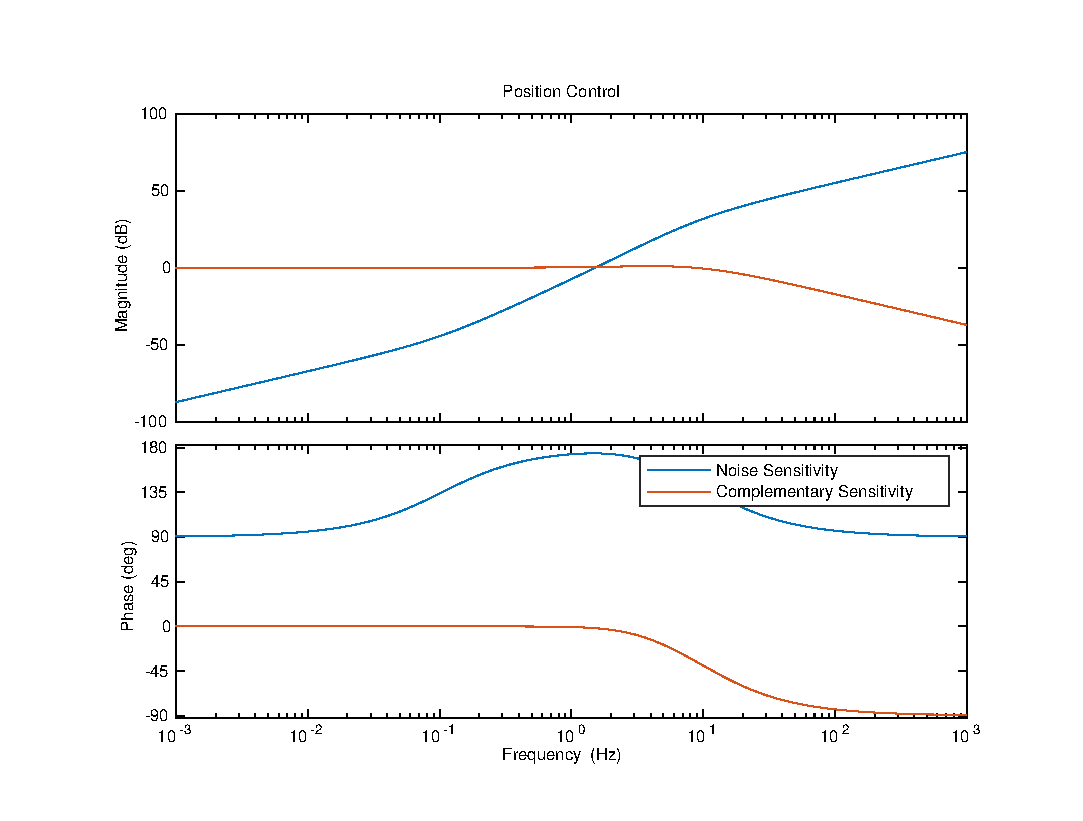
\includegraphics[width=0.8\textwidth]{images/position_tf.eps}
\end{center}
\caption{Position control bode plot of the complementary sensitivity function and noise sensitivity function}
\label{fig:position_tf}
\end{figure}


\begin{figure}[H]
\begin{center}
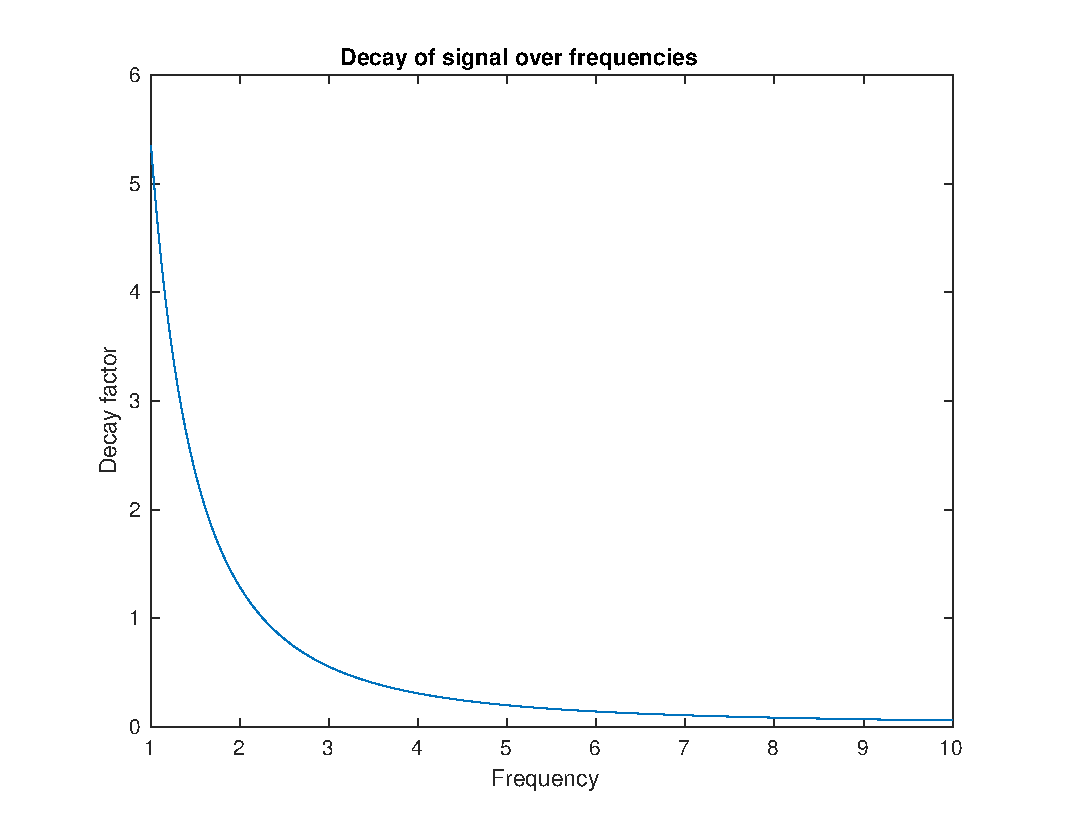
\includegraphics[width=0.8\textwidth]{images/decay.eps}
\end{center}
\caption{Linear decay factor obtained from $u_{sat}/CS(s)$ in the range of frequencies 1Hz to 10Hz}
\label{fig:position_ref}
\end{figure}

\newpage

\subsubsection{Modulated reference with original decay}
\noindent Let's try to see the result of this approach without smoothing of the magnitude decay. Originally the trasfer function $CS(s)$ tends to be really aggressive and cutting a lot of signal.

\begin{figure}[H]
\begin{center}
\hspace*{-5cm}
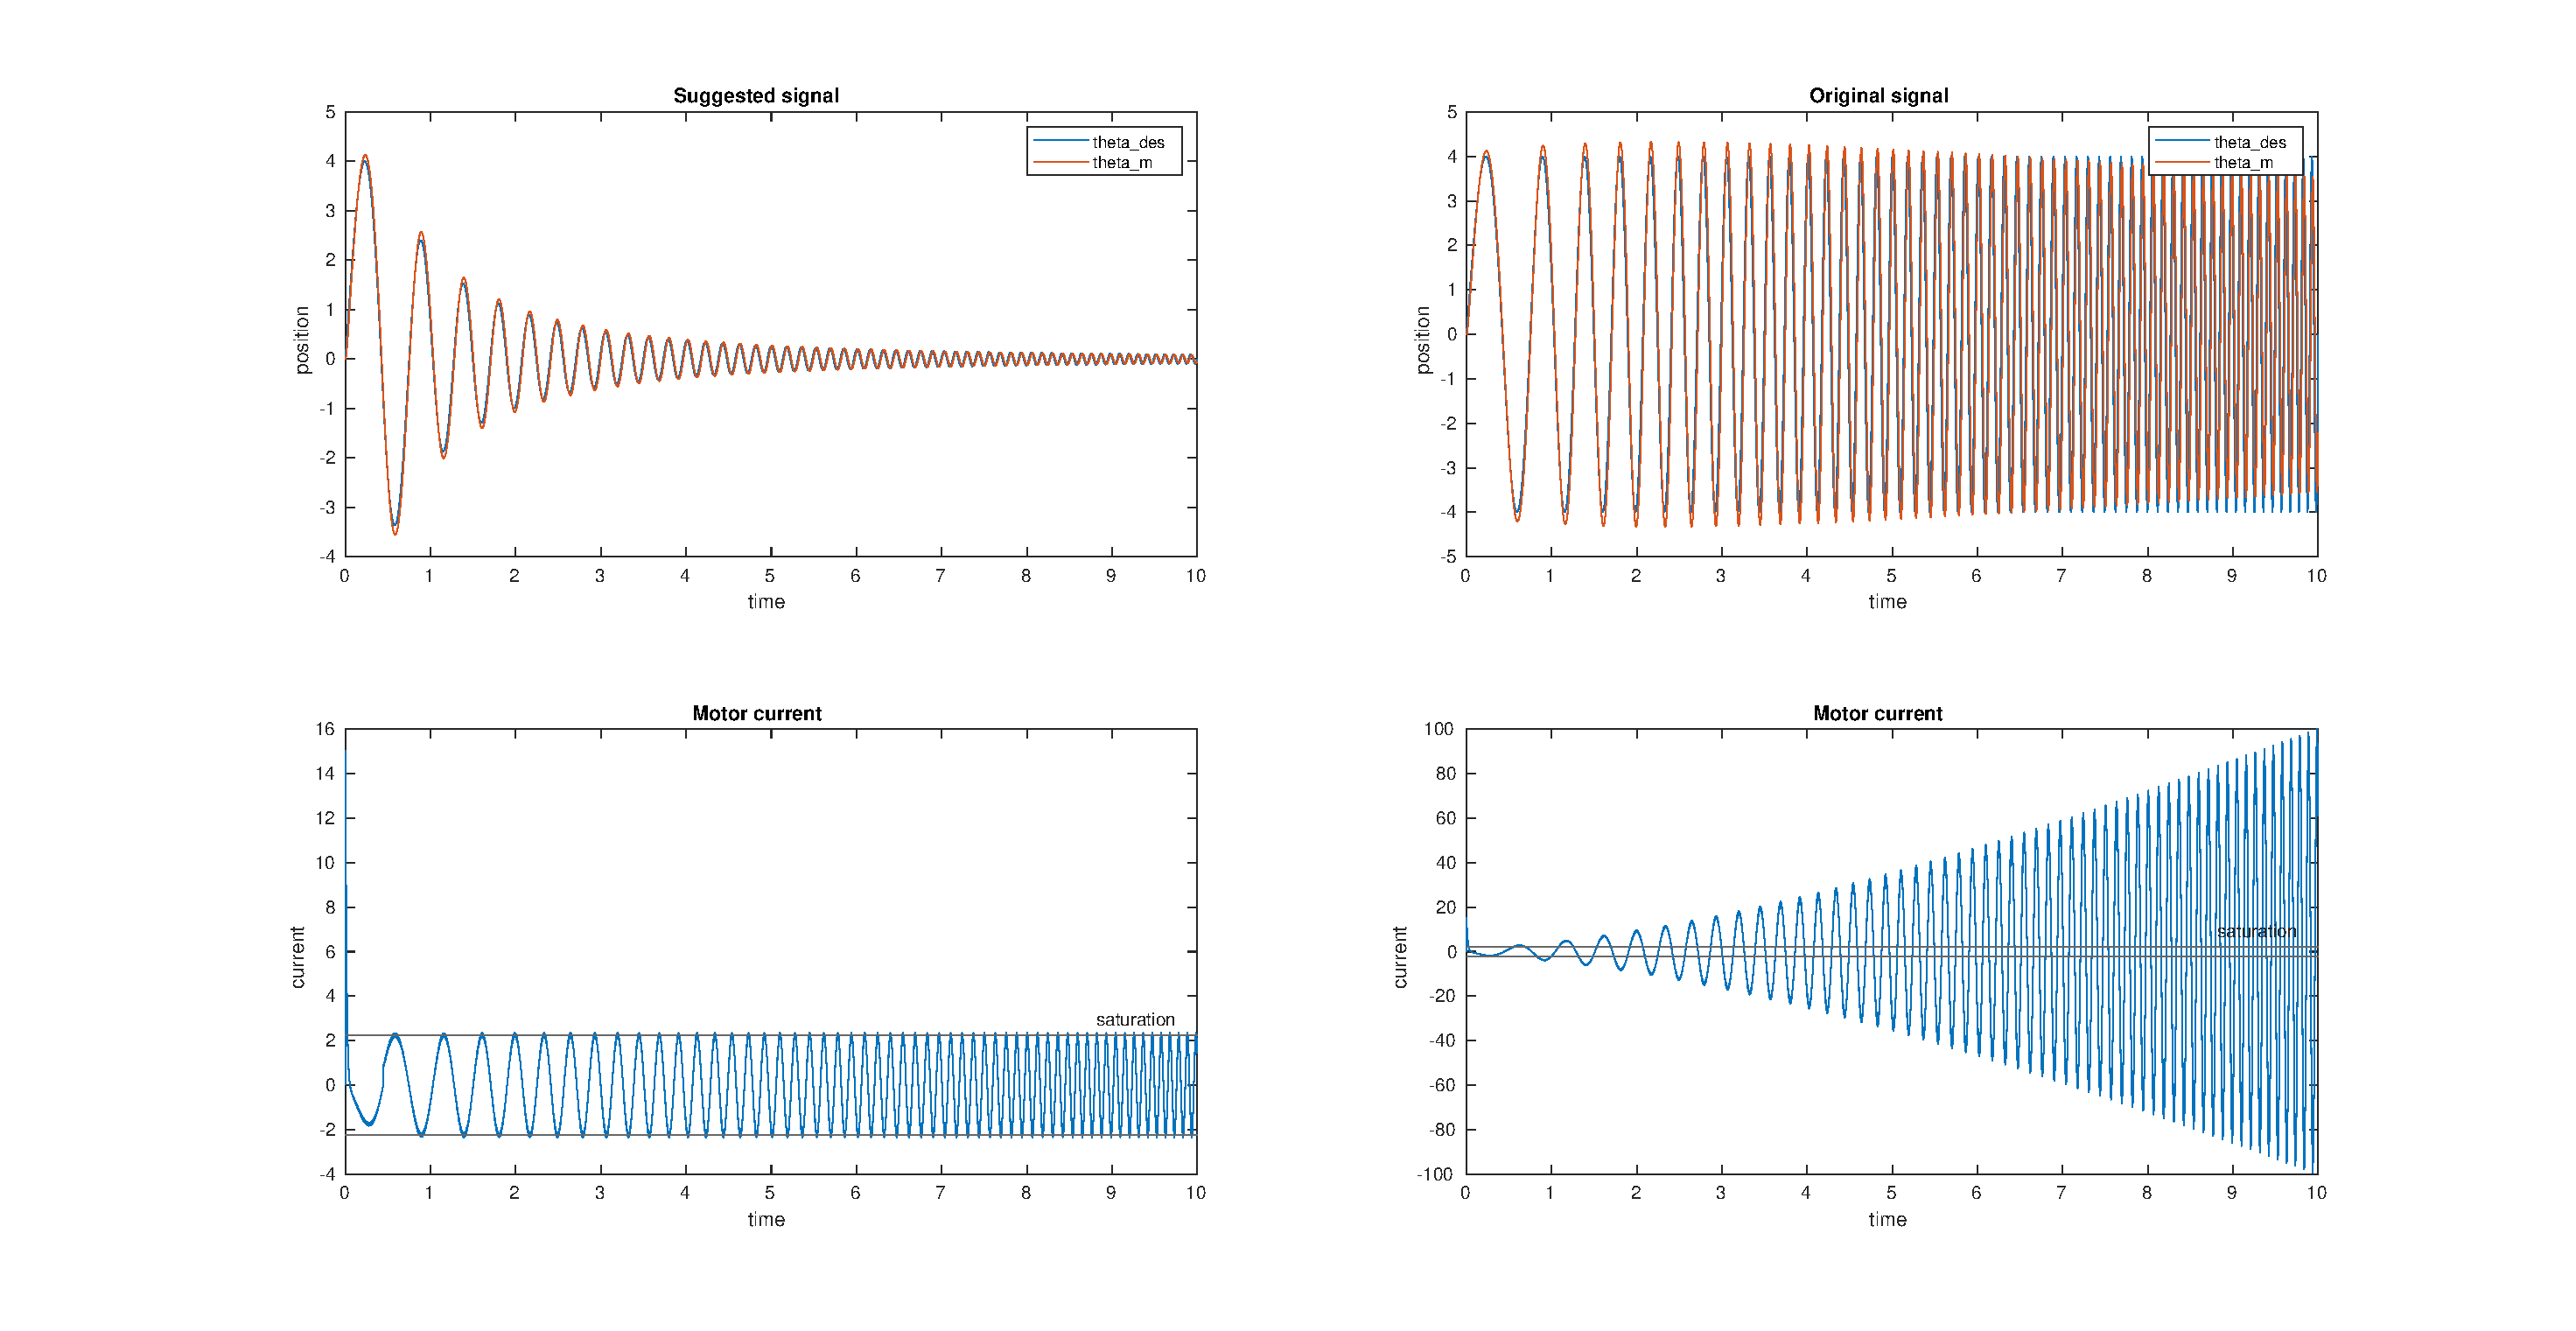
\includegraphics[width=1.6\textwidth]{images/position_tau2.eps}
\end{center}
\caption{Comparison of the original position signal with the suggested saturation aware one. In this case the original decay was used}
\label{fig:position_tau}
\end{figure}

What is visible is the fact that the decay is pretty agressive and it starts at 2Hz which is pretty early considering practical experiences of the motor data provided. In the following section we will try a modulated decay to improve the performances based on experiments on the trasfer function.

\newpage
\subsubsection{Modulated reference with augmented decay}
\noindent Let's compare the different responses we obtain using the original and the scaled signal, finally let's compare the actual current of the motor (saturation at $u_{sat} = 2.26$). The modulated decay is calculated as $modulated\_decay = exp(decay/20)$:

\begin{figure}[H]
\begin{center}
\hspace*{-5cm}
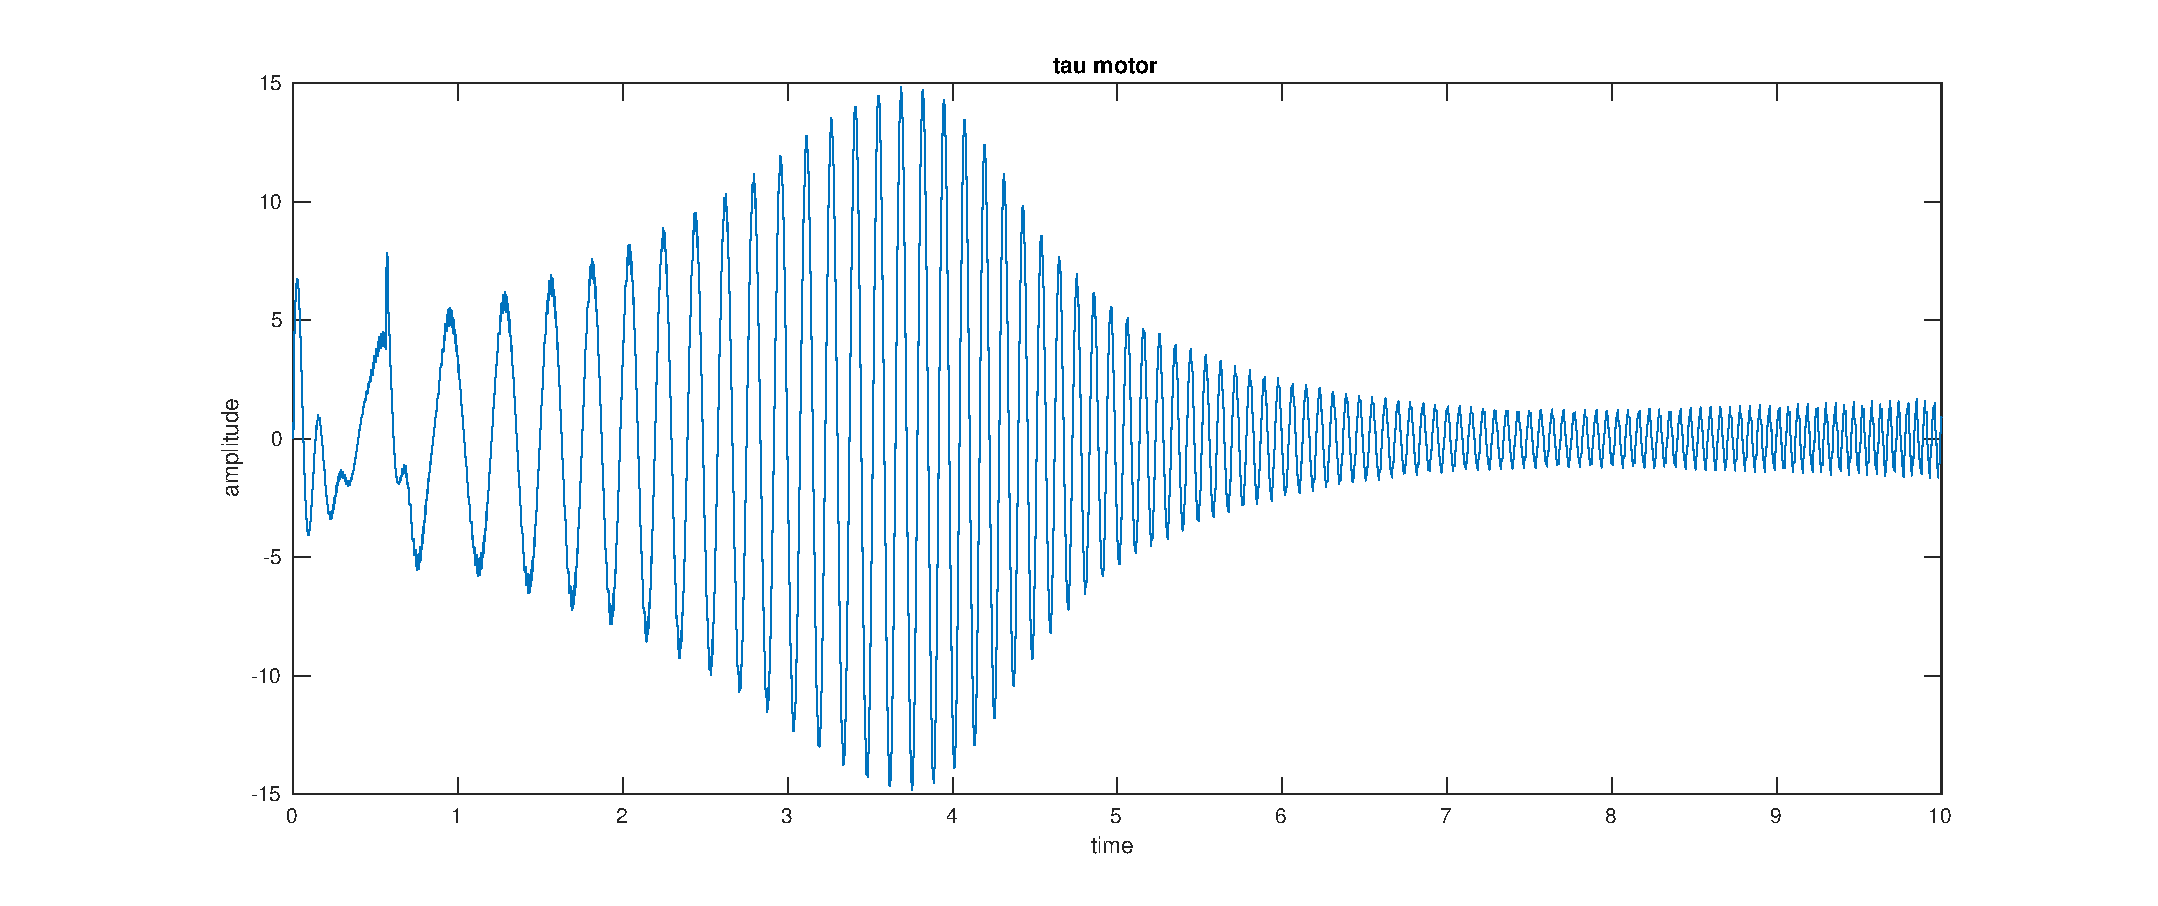
\includegraphics[width=1.6\textwidth]{images/position_tau.eps}
\end{center}
\caption{Comparison of the original position signal with the suggested saturation aware}
\label{fig:position_tau}
\end{figure}

\noindent The important aspect that plays an important role is the tuning of the controller which have to be appropriate, a sample is reported in Fig \ref{fig:position_step_response}. In case of bad tuning the suggested signal will be strongly deamplified as a result of considering a worst case scenario.

\begin{figure}[H]
\begin{center}
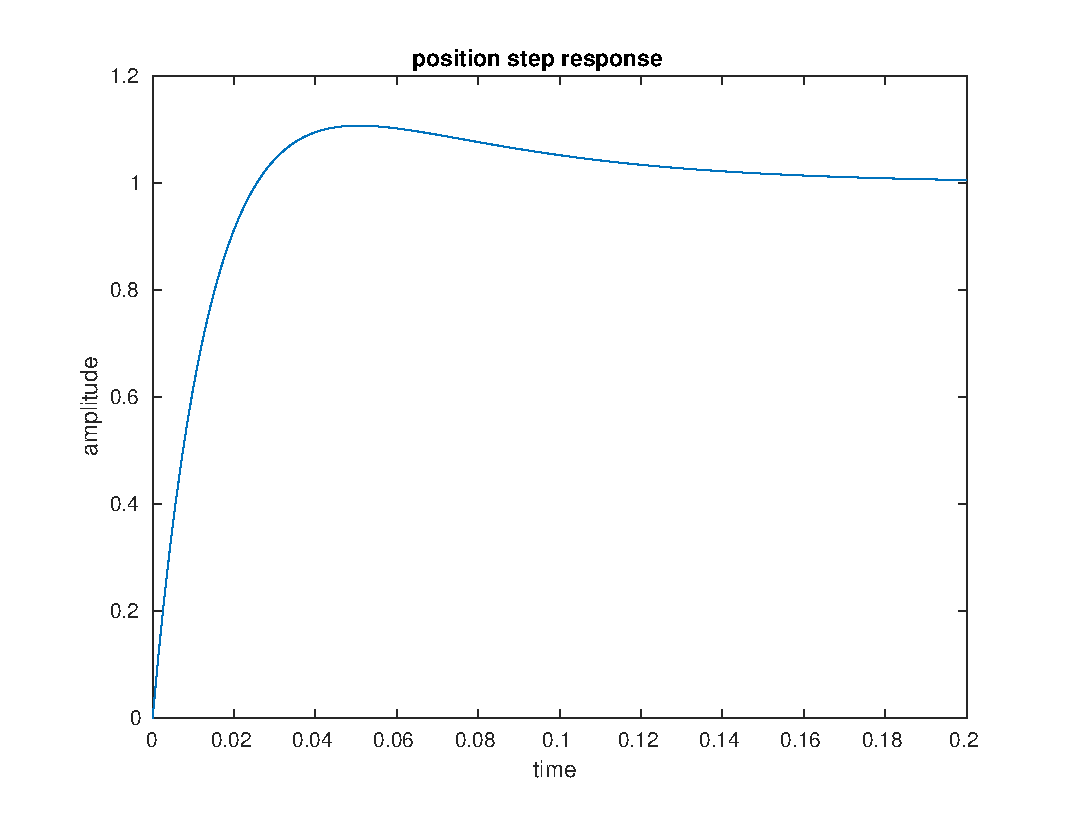
\includegraphics[width=0.3\textwidth]{images/position_step_resp.eps}
\end{center}
\caption{Step response of the system}
\label{fig:position_step_response}
\end{figure}
  
\newpage
\subsection{Force Control}
Let's consider a basic force control architecture for a linear motor model considering only the mechanical subsystem and a PD+FF controller. For simplicity only the environment stiffness $h$ (in rigid conditions):

\begin{figure}[H]
\begin{center}
\includegraphics[width=1\textwidth]{images/force.png}
\end{center}
\caption{Simulink model of force control architecture}
\label{fig:force_control}
\end{figure}

\noindent The related equations of the plant $P_l$ and the PD controller $C$ are:

\[
G = \frac{1}{\frac{J_m}{h}s^2 + \frac{d_m}{h}s + 1} \qquad
C = P + Ds;                             
\]

\bigskip
\noindent The two transfer functions $T(S)$ ($r$ to $y$) and $CS(s)$ ($r$ to $u$) are presented in Fig \ref{fig:force_tf} and the related original and suggested reference signal are reported in Fig \ref{fig:force_ref}. As it is visible the suggested approach is pretty aggressive especially due to the $epsilon$ considered in the $reference\_signal$ function presented above, moreover we are considering a worst case scenario.

\bigskip
\noindent To derive the $CS$ trasfer function the following equations were considered:

\[
  \tau_m = \tau_{des} + C(\tau_{des} - \tau_e)
\]
\[
  \tau_m = \tau_{des} + C\tau_{des} - \frac{CG(C+1)}{1+CG}\tau_{des}
\]
\[
  \tau_m = \bigg(1 + C - \frac{CG(1+C)}{1+CG}\bigg)\tau_{des}
\]

We can easily recognize $T$ as:
\[
  \tau_e = \frac{CG(1+C)}{1+CG}\tau_{des}
\]

\bigskip
\begin{figure}[H]
\begin{center}
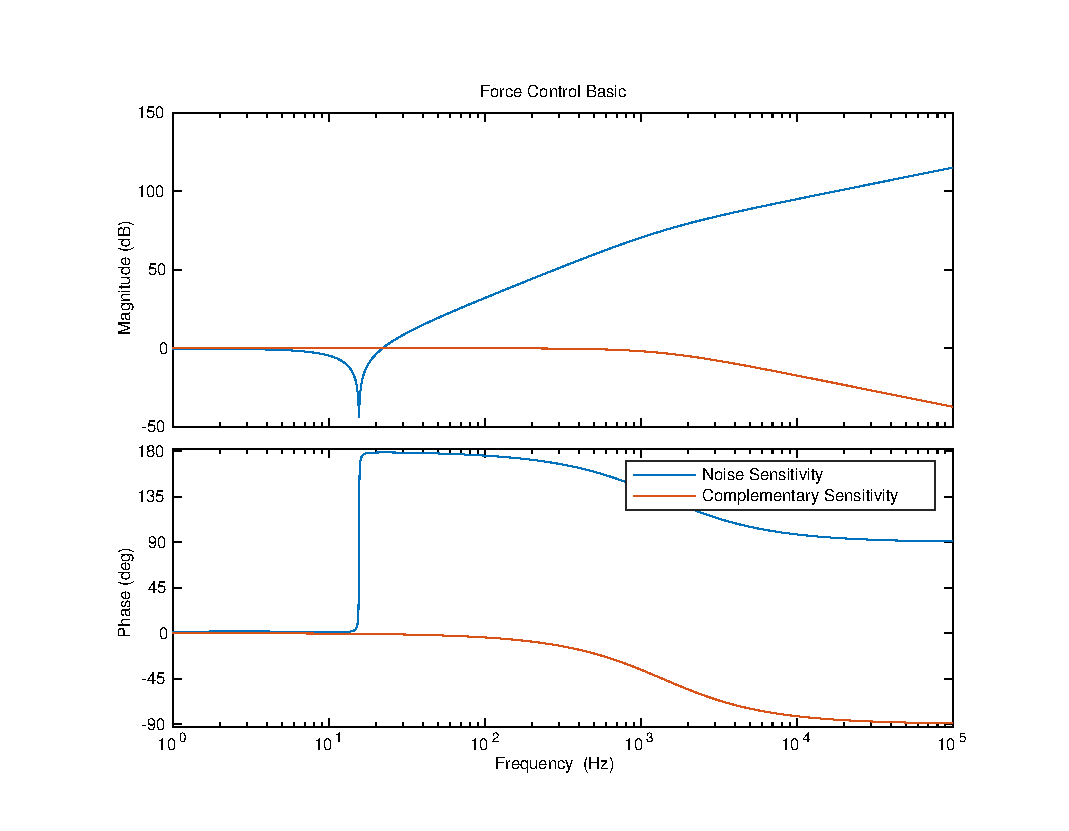
\includegraphics[width=0.8\textwidth]{images/force_tf.eps}
\end{center}
\caption{Force control bode plot of the complementary sensitivity function and noise sensitivity function}
\label{fig:force_tf}
\end{figure}


\begin{figure}[H]
\begin{center}
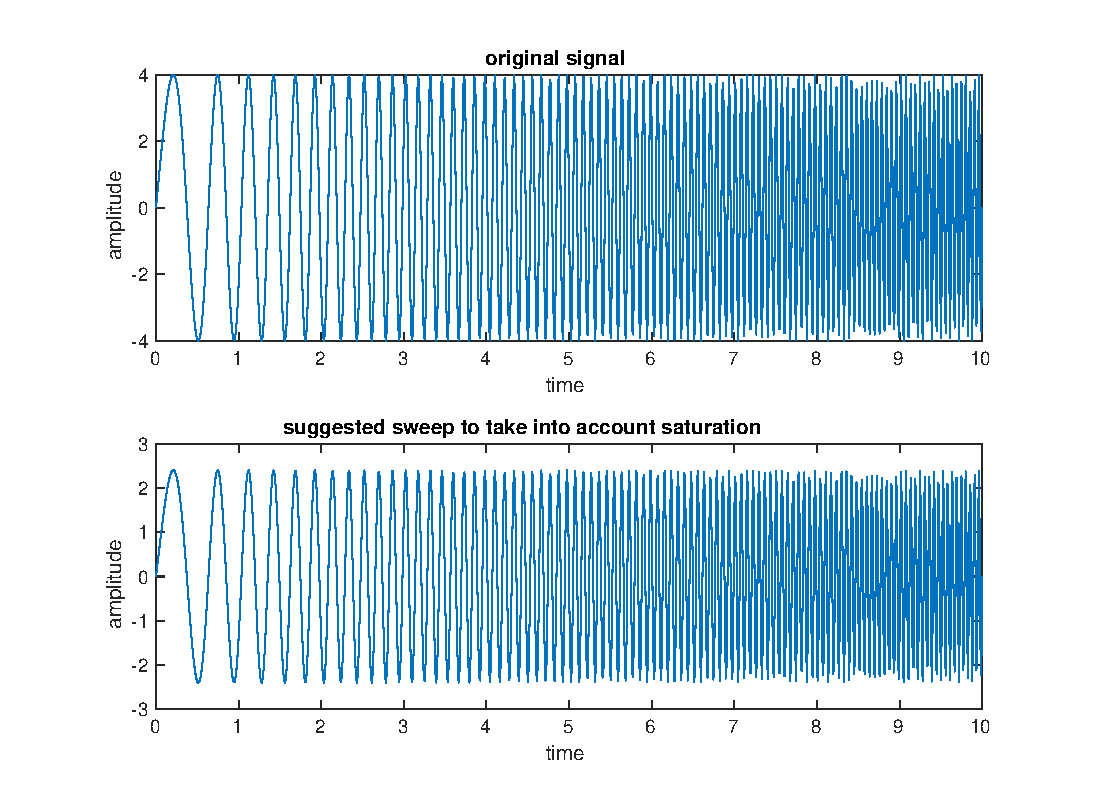
\includegraphics[width=0.8\textwidth]{images/force_scaled.eps}
\end{center}
\caption{original and scaled sweep for the force reference. As it is visible we have a different behaviour than the position control due to a completly different $CS(s)$ transfer function}
\label{fig:force_ref}
\end{figure}

\noindent Let's compare the different responses we obtain using the original and the scaled signal, finally let's compare the actual current of the motor (saturation at $u_{sat} = 2.26$) :

\begin{figure}[H]
  \begin{center}
  \hspace*{-5cm}
  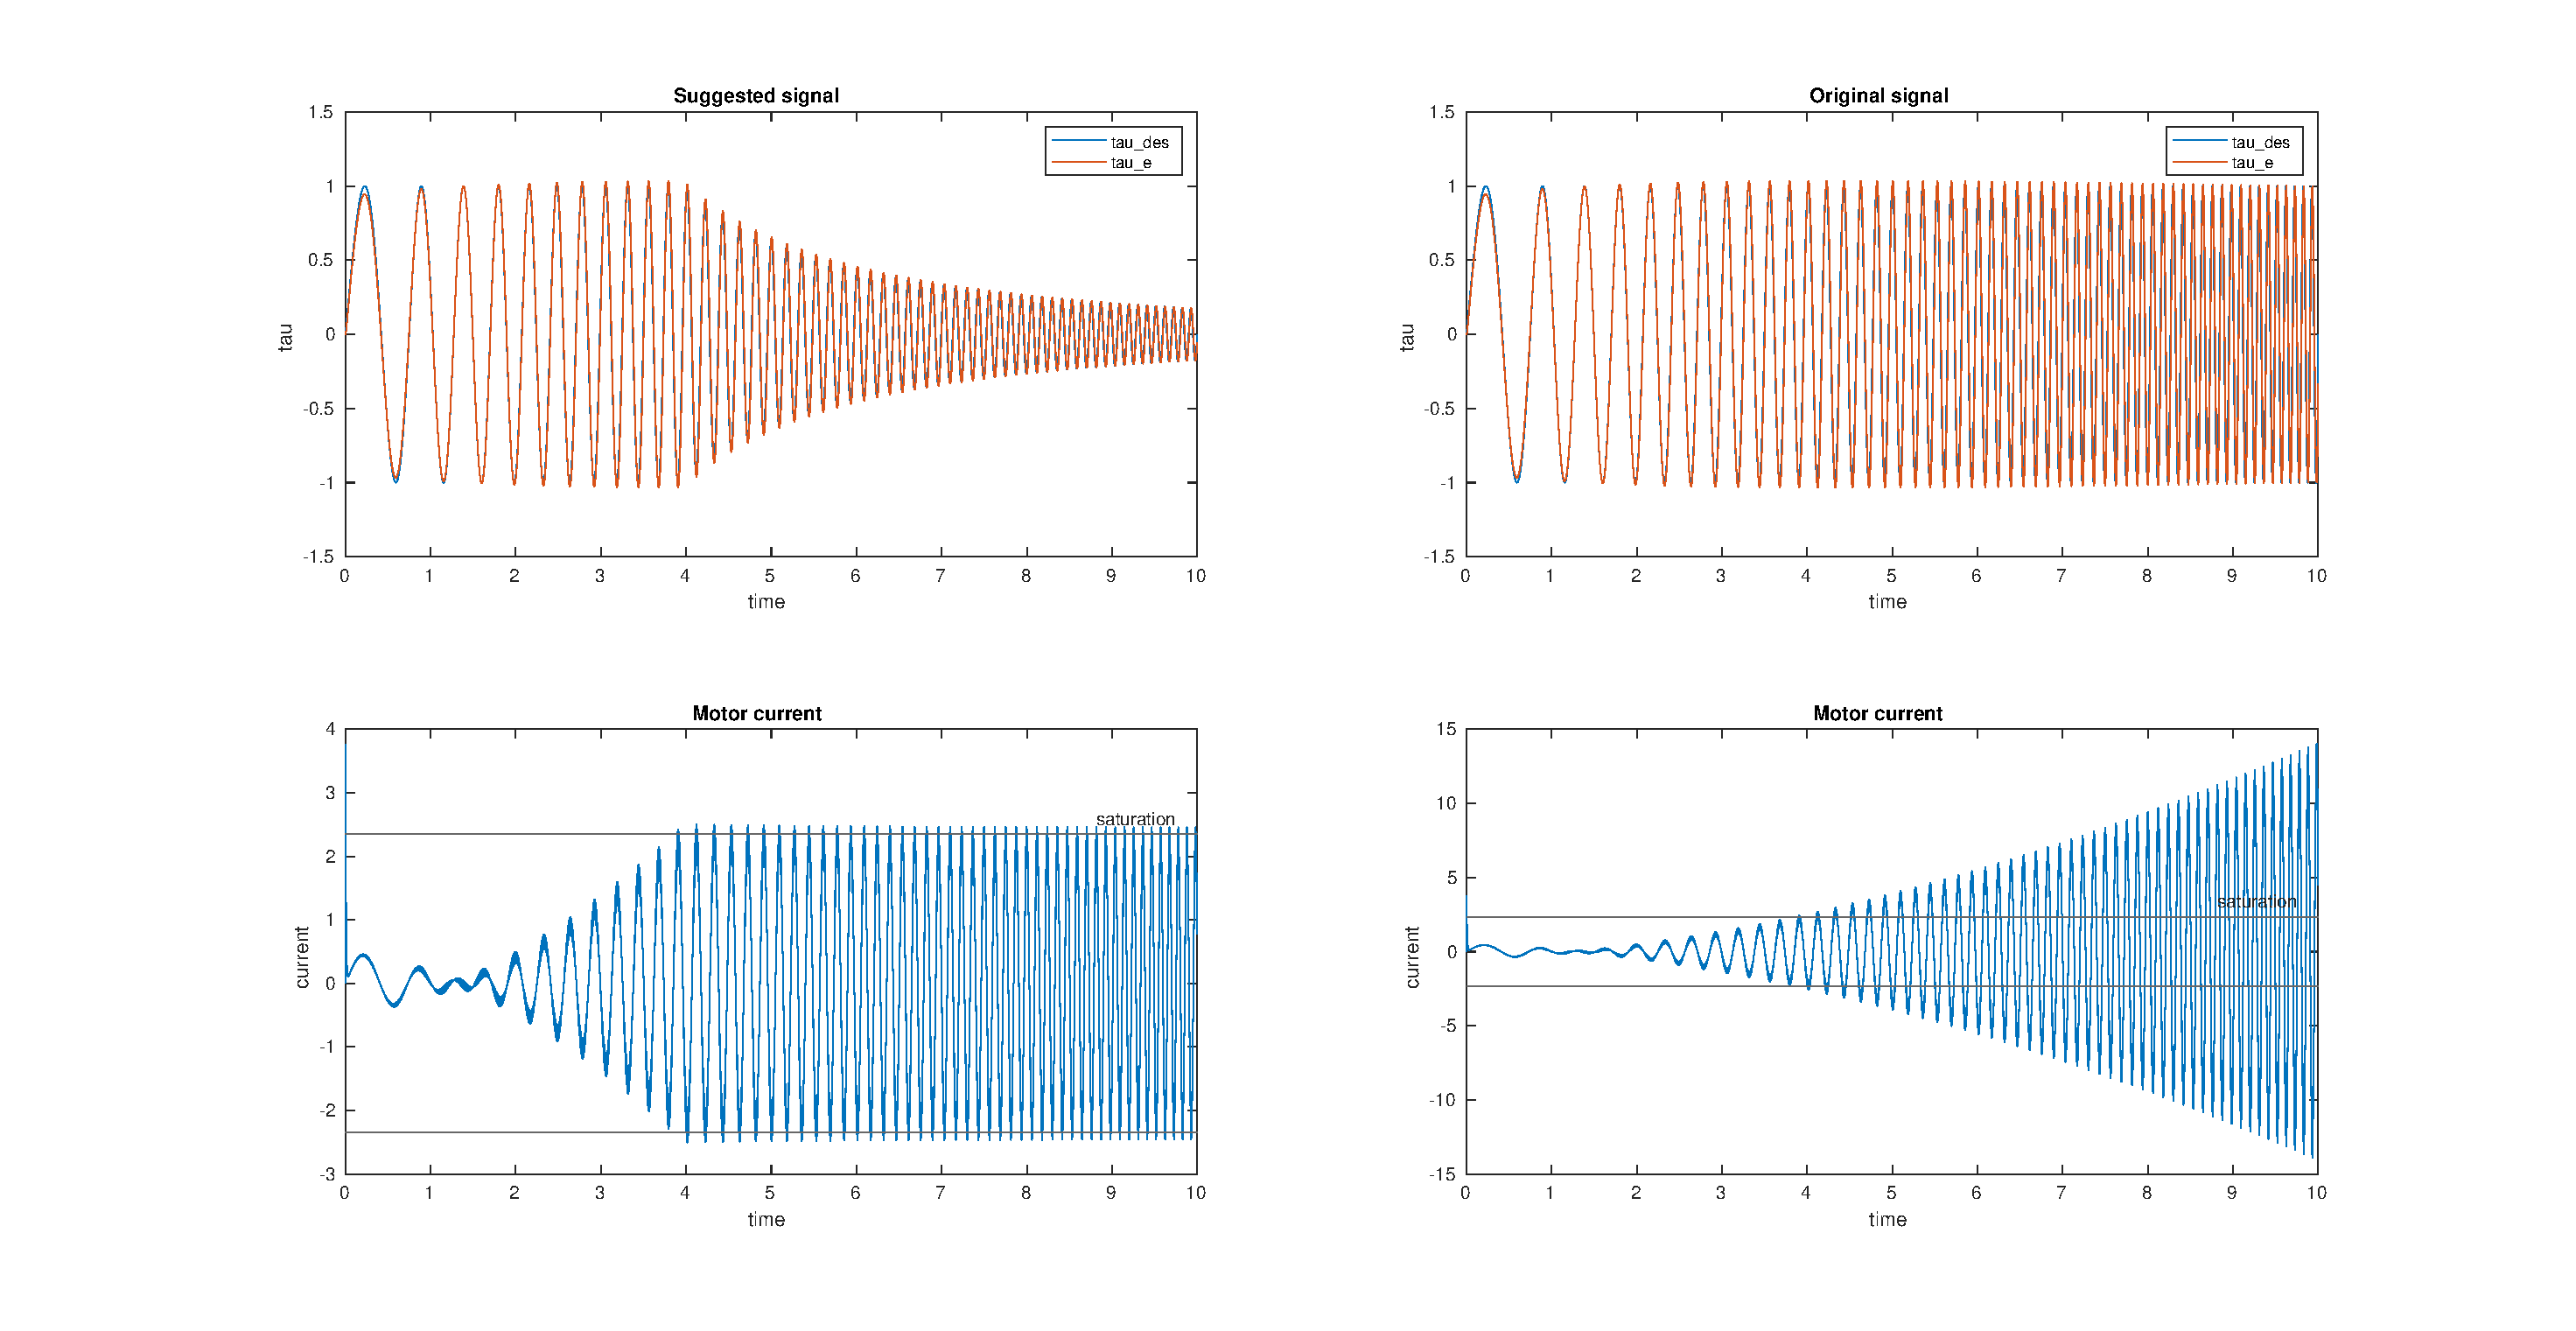
\includegraphics[width=1.6\textwidth]{images/force_tau.eps}
  \end{center}
  \caption{Comparison of the original force signal with the suggested saturation aware}
  \label{fig:force_tau}
  \end{figure}

\section{Limitations}

The current approach based on the use of the transfer function $CS(s)$ has lots of limitations:
\begin{itemize}
  \item The approach assumes full knowledge of the considered system, everything has to be identified correctly and this is even a bigger limitation for force control because we don't have informations about the environment which makes the use of the transfer functions not reliable at all.
  \item We assume a linear system which is a big limitation since it doesn't consider non-linear behaviours of the DC motors. For this cases having at least one real experiment to validate the data is a must.
  \item The use of $CS(s)$ is not reliable in some scenarios due to accentuated shapes of the transfer function in Fig \ref{fig:sea_tf} the transfer function of a SEA with links is reported as well as its relevant equations.
\end{itemize}

\begin{figure}[H]
\begin{center}
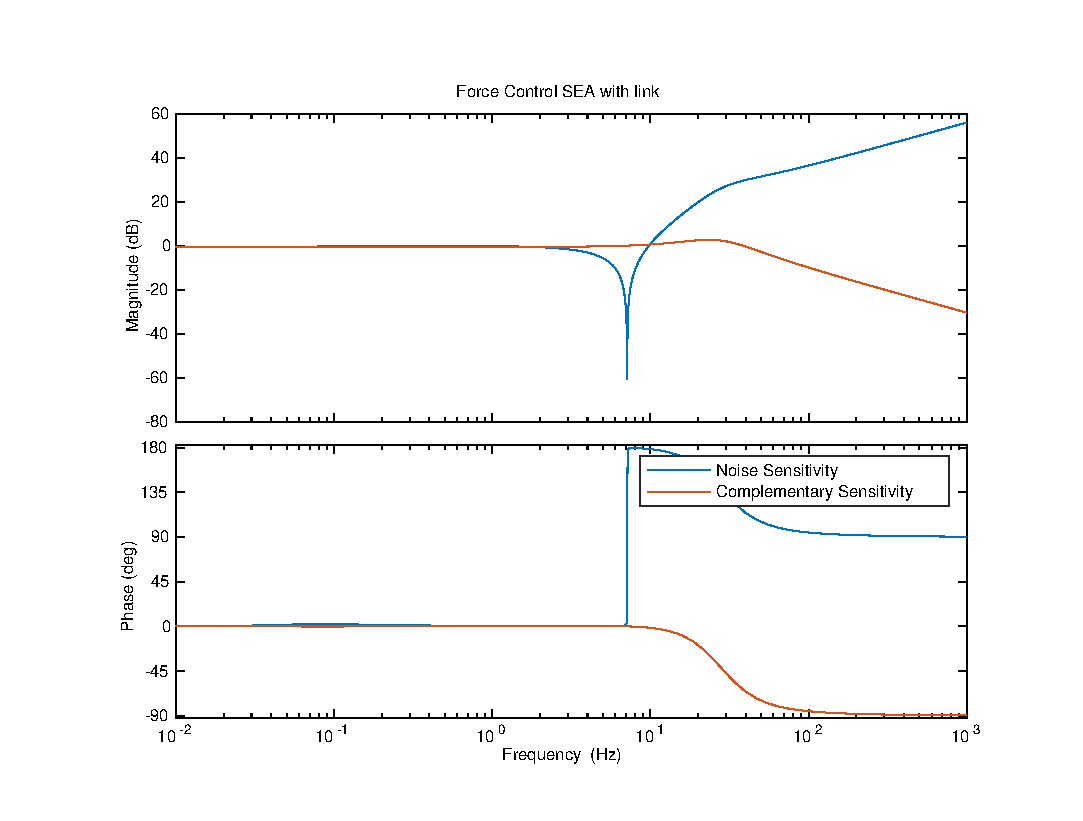
\includegraphics[width=0.8\textwidth]{images/sea_tf.eps}
\end{center}
\caption{SEA with link force control bode plot of the complementary sensitivity function and noise sensitivity function}
\label{fig:sea_tf}
\end{figure}

\[
  r = \frac{Ks}{Ke} \qquad
  E = \frac{J_e}{K_e}s^2 + \frac{B_e}{K_e}s + 1;
\]\[
  F = \frac{E}{(E + r)\frac{J_m}{K_s}s^2 + E} \qquad
  C = P + Ds;    
\]

\section{Other approaches}

Simulating the experiments in simulink is in general a good way to verify the presence of saturation but it is affected by the same problems related to prior knowledge and linear behaviours (at least without implementing a non-linear system). A good way to generate a current saturation aware reference signal is adapting the reference in real time by reading directly the current provided to the motor. If this exceeds a certain threasold just drop a certain percentage. With this approach we can't know a priori the "amplitude shape" of the signal but it will be recovered after the experiments (using the log captured by the Forecast system). The bandwith estimation can be performed using the Matlab toolbox over that data.

\section{Conclusions}
The report is an attempt to provide a way to generate current saturation aware signals using noise sensitivity trasfer function. The basic idea was provided as well as some simulation results. The main limitations and other possibilities were discussed and analysed.

\begin{thebibliography}{9}

\bibitem{Forecast}
Forecast Project https://eurobench2020.eu/developing-the-framework/force-control-algorithms-testbench-forecast/

\bibitem{scientist}
Karl Johan Astrom, Richard M. Murray Feedback Systems An Introduction for Scientists and Engineers
\end{thebibliography}

\end{document}


